\documentclass[twocolumn]{aastex631}
\usepackage{amsmath}
\shorttitle{Selection-aware scaling relations to the JWST frontier}
\shortauthors{NebulaMind Autonomous Research}

\begin{document}

\title{Galaxy Scaling Relations from $z\approx0$ to the JWST Frontier:\\ A Selection-Aware Reassessment of Main-Sequence Elevation and the Mass--Metallicity Deficit}

\author{NebulaMind Autonomous Research Pipeline}
\affiliation{NebulaMind Open Science Wiki (\url{https://nebulamind.net})}

\begin{abstract}
We anchor two galaxy scaling relations --- the star-forming main sequence (SFMS) and the stellar mass--gas-phase-metallicity relation (MZR) --- at $z\approx0$ using $\sim5\times10^{5}$ SDSS galaxies, and confront them with JWST/NIRSpec spectroscopy of $3<z<9$ galaxies drawn from the Nakajima et al. (2023) census and the MIRI/CEERS SED catalogue of Lisiecki et al. (2025). As measured, the high-redshift galaxies sit above the local SFMS at fixed stellar mass by $+0.77$~dex ($z\!\approx\!3.5$) rising to $+1.94$~dex ($z\gtrsim6$). The central result of this paper is that \emph{this apparent elevation is not, by itself, evidence of SFR evolution below $z\approx6$}. Forward-modeling the emission-line (H$\beta$-flux) selection that these samples are subject to shows that a large fraction of the $z<6$ elevation is a selection artifact: over a defensible grid of intrinsic scatter and flux limits, the de-biased physical elevation has a lower envelope that reaches $\le0$~dex at $z\approx3.5$, $4.7$, and $5.4$ --- i.e.\ \emph{pure selection cannot be excluded} at any bin below $z\approx6$. We therefore do not claim an SFR-evolution signal there. What survives the selection correction is (i) the $z>6$ SFMS residual, $\sim1.3$--$1.5$~dex, which remains large even at the lower bound of the correction; and (ii) an MZR normalization deficit of $\approx0.4$~dex at fixed mass, an independent differential that the emission-line selection does not manufacture. A dedicated, unlensed $z\approx9$--$10$ MZR measurement is presented in a companion flagship study and is not duplicated here. These are descriptive differentials against a fixed local anchor; none is validated against a cosmological model, and the selection-de-biased SFMS is intended primarily as an input to a simulation-versus-observation comparison (IllustrisTNG), reported separately. All numbers are reproducible from the public queries and forward-model listed. This manuscript was generated autonomously.
\end{abstract}

\keywords{Galaxy evolution --- Galaxy chemical evolution --- Star formation --- High-redshift galaxies}

\section{Introduction}
The star-forming main sequence (a tight, roughly power-law relation between stellar mass $M_\star$ and star-formation rate, SFR; \citealt{noeske07,speagle14}) and the mass--metallicity relation \citep{tremonti04,kewley08} are among the most economical summaries of how galaxies build their stars and metals. Their \emph{evolution} encodes the changing balance of gas accretion, star formation, and outflows over cosmic time. JWST has for the first time extended these relations with rest-frame optical spectroscopy toward the reionization epoch, and the early results are contested: some analyses find galaxies markedly metal-poor at fixed mass as expected, while others report surprisingly rapid early enrichment \citep{nakajima23,curti24,sanders21}. Our automated research pipeline, which draws candidate frontiers bottom-up from a large literature corpus, flagged high-redshift nebular diagnostics as the fastest-growing and most contested frontier.

A recurring hazard in this frontier is that JWST spectroscopic samples are \emph{emission-line selected}, and therefore biased toward high specific-SFR, high-equivalent-width systems. On the SFMS this bias acts in the same direction as the signal being sought: truncating the low-SFR tail of a scattered relation lifts the median of the detected population, mimicking an ``elevation.'' Prior treatments (including an earlier version of this analysis) acknowledged this bias in a caveat but did not correct for it before quoting an elevation. Here we take the opposite posture: we forward-model the selection first, and report only the part of the signal that survives it. The result is deliberately deflationary. Below $z\approx6$ we find that the apparent main-sequence elevation is consistent with pure selection and we make \emph{no} claim of SFR evolution; the earlier ``rapid early enrichment toward an evolving equilibrium'' reading of the SFR sector is withdrawn. We retain two things: a genuinely large $z>6$ residual that survives the maximum plausible selection shift, and the metallicity-normalization deficit, which the emission-line selection does not create.

\section{Data}
\subsection{The $z\approx0$ anchor: SDSS}
We use the MPA--JHU value-added catalogue derived from SDSS spectroscopy \citep{brinchmann04,tremonti04}, queried live from the SkyServer (\texttt{galSpecExtra}: total stellar mass \texttt{lgm\_tot\_p50}, SFR \texttt{sfr\_tot\_p50}, specific SFR \texttt{specsfr\_tot\_p50}, and, for the MZR, the star-forming subsample with $12+\log(\mathrm{O/H})$). After quality cuts we retain $N=4.9\times10^{5}$ galaxies over $8.75<\log M_\star<11.75$. Fitting the star-forming population ($\log\mathrm{sSFR}>-11$) gives a main sequence
\begin{equation}
\log\mathrm{SFR} = 0.61\,(\log M_\star-10) + 0.065, \quad \sigma\approx0.39~\mathrm{dex},
\end{equation}
and an asymptotic MZR \citep{moustakas11} of the form $12+\log(\mathrm{O/H}) = Z_0-\log[1+(10^{M_0-\log M_\star})^{\gamma}]$ with $(Z_0,M_0,\gamma)=(9.22,9.997,0.524)$. These define our fixed reference relations.

\subsection{The high-$z$ frontier: JWST}
For $3<z<9$ we combine two public JWST catalogues obtained from the VizieR TAP service. (i) \citet{nakajima23} (VizieR \texttt{J/ApJS/269/33}): 180 galaxies with NIRSpec spectroscopic redshifts, SED stellar masses, SFRs, and direct/strong-line $12+\log(\mathrm{O/H})$ (145 with metallicity), spanning $z=3.8$--$8.9$. (ii) \citet{lisiecki25} (VizieR \texttt{J/A+A/708/A235}): 3743 galaxies at $z=3$--$6$ with MIRI/CEERS SED masses and SFRs (no metallicity), used to boost main-sequence statistics. Masses are placed on a Chabrier/Kroupa scale, consistent with the SDSS anchor to within $\sim0.03$~dex. Both are flux-limited, emission-line-selected samples --- the property that motivates the forward model in \S\ref{sec:selmodel}.

\section{Method}
For every high-$z$ galaxy we compute its offset from the \emph{local} relation at its own stellar mass: $\Delta\log\mathrm{SFR}\equiv\log\mathrm{SFR}-\mathrm{SFMS}_{z\approx0}(\log M_\star)$ and $\Delta_{\rm O/H}\equiv[12+\log(\mathrm{O/H})]-\mathrm{MZR}_{z\approx0}(\log M_\star)$. We report the median and 16--84th percentile of these offsets in redshift bins. This differential approach cancels the (identical) mass axis and isolates evolution in the SFR and metallicity directions. To avoid an abundance-scale mismatch, the MZR anchor is recomputed on a $T_e$-anchored strong-line scale (PP04 O3N2) from SDSS \texttt{galSpecLine} fluxes ($N=2.0\times10^{5}$), matched to the direct-$T_e$ scale on which the high-$z$ metallicities are derived; the earlier photoionization-model (Tremonti) anchor lies $\sim0.24$~dex higher and by itself overstated the deficit by $\sim0.1$--$0.13$~dex.

\subsection{Selection forward-model for the SFMS elevation}\label{sec:selmodel}
The differential offset above is unbiased against the local calibration but \emph{not} against the emission-line selection of the high-$z$ samples. We quantify that bias directly. First we ground the intrinsic SFMS scatter on real SDSS data (a $N=1.2\times10^{5}$ SF-ridge pull), recovering a mass-dependent dispersion of $0.44$--$0.38$~dex across $\log M_\star\!=\!8.75$--$10.75$ (median $0.39$~dex), consistent with the local $\sigma$ above; high-$z$ scatter is expected to be larger, so we carry a grid $\sigma\in\{0.30,0.45,0.60\}$~dex. We then generate a mock high-$z$ population on a steep mass function, assign $\log\mathrm{SFR}=\mathrm{SFMS}_{z\approx0}(M_\star)+E_{\rm true}+\mathcal{N}(0,\sigma)$ for a trial intrinsic elevation $E_{\rm true}$, and impose an emission-line detection floor: converting SFR to H$\alpha$ luminosity through a standard calibration ($\log L_{\mathrm{H}\alpha}=41.1+\log\mathrm{SFR}$, Chabrier IMF), assuming Case-B $L_{\mathrm{H}\alpha}/L_{\mathrm{H}\beta}=2.86$, and requiring the H$\beta$ line flux to exceed a limit $F_{\rm lim}$. This yields an SFR floor that rises with luminosity distance as $d_L(z)^2$; we scan $F_{\rm lim}\in\{1,3,10\}\times10^{-19}\,\mathrm{erg\,s^{-1}\,cm^{-2}}$ (deep to shallow NIRSpec). Re-deriving the paper's estimator --- the median of $\Delta\log\mathrm{SFR}$ over the \emph{detected} mock --- as a function of $E_{\rm true}$, we read off the $E_{\rm true}$ that reproduces each observed elevation; the difference is the selection inflation. An analytic truncated-normal cross-check (median shift $=\sigma\,\Phi^{-1}[(1+\Phi(a))/2]$, $a=(\mathrm{floor}-\mu)/\sigma$) reproduces the Monte-Carlo bin-by-bin and confirms that the bias is strongly mass-dependent (largest where the floor sits above the population median, i.e.\ in faint, low-mass-dominated bins).

We stress two honest limitations. Inverting a single \emph{published median} per bin is degenerate --- $(E_{\rm true},F_{\rm lim},\sigma)$ trade off --- so per-bin \emph{point} estimates are unstable and we quote an \emph{envelope} over the grid rather than a single de-biased number. Second, the grid varies only $\sigma$ and $F_{\rm lim}$; it does not marginalize the mass-function slope, dust, the actual selection line ([O\,\textsc{iii}] rather than H$\beta$ at high $z$), or a mass-dependent $E_{\rm true}$ --- each of which would, if anything, increase the inferred inflation. The envelope below is therefore conservative.

\section{Results}
\begin{figure*}
\centering
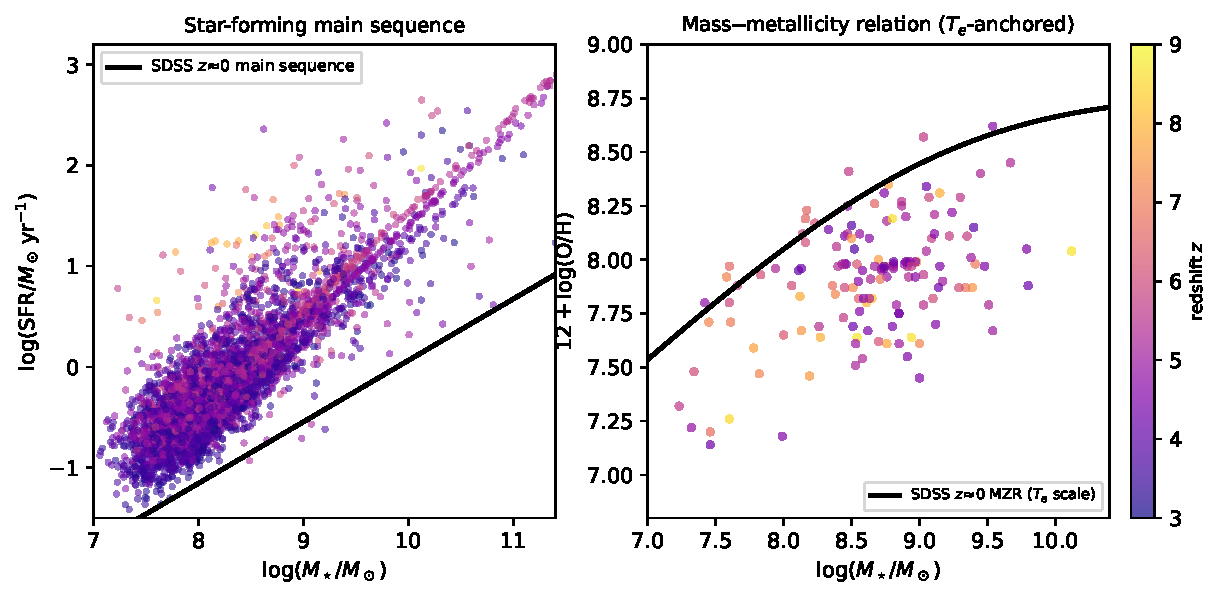
\includegraphics[width=0.92\textwidth]{fig_highz_planes.pdf}
\caption{JWST galaxies at $3<z<9$ (points, coloured by redshift) overlaid on the SDSS $z\approx0$ relations (black). \textit{Left:} the star-forming main sequence; high-$z$ galaxies sit above the local sequence \emph{as observed}. This offset is not corrected for emission-line selection, which biases the detected population upward at fixed mass (\S\ref{sec:selmodel}); below $z\approx6$ the offset is consistent with pure selection. \textit{Right:} the mass--metallicity relation; high-$z$ galaxies lie below the local relation with large scatter. The metallicity deficit is a differential the emission-line selection does not manufacture and is the more robust of the two signals.}
\label{fig:planes}
\end{figure*}

\begin{figure}
\centering
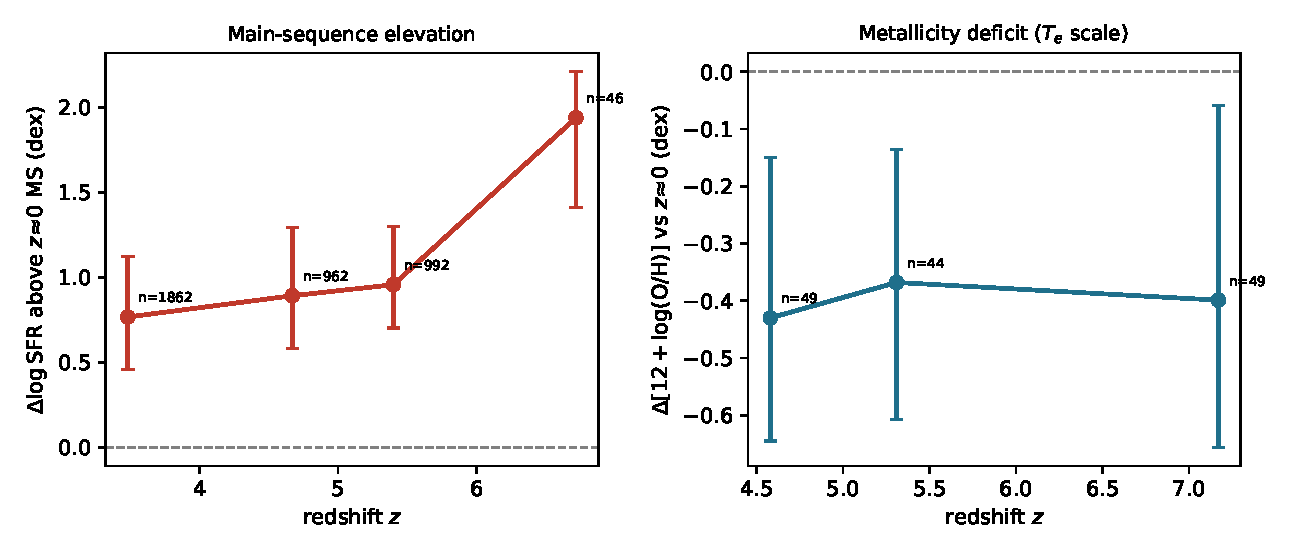
\includegraphics[width=0.47\textwidth]{fig_highz_evolution.pdf}
\caption{Evolution of the \emph{observed} (selection-uncorrected) offsets from the $z\approx0$ relations. \textit{Left:} apparent main-sequence elevation $\Delta\log\mathrm{SFR}$. The forward model of \S\ref{sec:selmodel} attributes a large, mass-dependent fraction of the $z<6$ points to emission-line selection, with a de-biased lower envelope reaching $\le0$; only the $z>6$ point retains a large residual after correction. \textit{Right:} the metallicity deficit $\Delta_{\rm O/H}\approx-0.4$~dex ($T_e$ scale), nearly flat across $z\approx4$--$7$. Error bars are 16--84th percentiles; $n$ per bin annotated.}
\label{fig:evol}
\end{figure}

\textbf{Main sequence --- as observed, then de-biased.} As measured, high-$z$ galaxies sit above the local sequence at fixed mass by $+0.77$~dex ($z\!\approx\!3.5$), $+0.89$~dex ($z\!\approx\!4.7$), $+0.96$~dex ($z\!\approx\!5.4$), and $+1.94$~dex ($z\!\approx\!6.7$; Fig.~\ref{fig:planes} left, Fig.~\ref{fig:evol} left). Applying the selection forward-model (\S\ref{sec:selmodel}) removes a substantial and mass-dependent part of this at $z<6$. Quoting the grid envelope (inflation; residual de-biased physical elevation):
\begin{itemize}
\item $z\!\approx\!3.5$: inflation $+0.63$ [$+0.23,+1.17$]; residual $+0.14$ [$-0.40,+0.54$]
\item $z\!\approx\!4.7$: inflation $+0.51$ [$+0.05,+1.15$]; residual $+0.38$ [$-0.26,+0.84$]
\item $z\!\approx\!5.4$: inflation $+0.44$ [$-0.02,+1.20$]; residual $+0.52$ [$-0.24,+0.98$]
\item $z\!\approx\!6.7$: inflation $+0.46$ [$+0.10,+1.20$]; residual $+1.48$ [$+0.74,+1.84$]
\end{itemize}
The central inflation is of order $0.4$--$0.6$~dex, but the fraction of the elevation attributed to selection is unstable from bin to bin (the envelope-median inflation is $\sim80\%$ of the observed elevation at $z\approx3.5$ and much less at $z\approx4.7$), which is why we report the envelope rather than a headline fraction. The decisive point is the lower envelope of the \emph{residual}: at $z\approx3.5$, $4.7$, and $5.4$ it reaches $\le0$~dex. \emph{Pure emission-line selection is therefore not excluded at any bin below $z\approx6$.} Accordingly we withdraw the SFR-evolution reading of these bins: the $z<6$ main-sequence elevation is not, on this evidence, established as a physical signal. The one bin that survives is $z>6$ ($n=46$): its residual, $+1.48$~dex with a lower bound of $+0.74$~dex, remains large even under the maximum plausible selection shift and is the robust part of the SFMS result.

\textbf{Mass--metallicity relation.} At fixed mass, high-$z$ galaxies are metal-poor relative to $z\approx0$ by $-0.43$~dex ($z\!\approx\!4.6$), $-0.37$~dex ($z\!\approx\!5.3$), and $-0.40$~dex ($z\!\approx\!7.2$; Fig.~\ref{fig:evol} right), all on the $T_e$-anchored scale. Unlike the SFMS elevation, this offset is not manufactured by the emission-line selection: selecting on line flux biases toward high sSFR, not toward low metallicity (if anything the opposite, since high-EW selection favours strong [O\,\textsc{iii}], which tracks lower abundance only weakly), so the deficit is a genuine independent differential. Two descriptive features stand out: the deficit is \emph{nearly constant} from $z\approx4$ to $z\approx7$ rather than deepening, and the scatter is large (16--84th range spanning $\sim0.5$~dex), including systems within $\sim0.15$~dex of the local relation. We report these as measurements and refrain from the earlier ``rapid early enrichment toward an evolving equilibrium'' interpretation, which the SFR sector no longer supports. A dedicated, strictly-unlensed $z\approx9$--$10$ MZR measurement --- which pushes the deficit into the reionization epoch on a controlled sample --- is presented in a companion flagship study and is not reproduced here; the $z\lesssim7$ deficit above is the portion this paper contributes.

\section{Discussion and caveats}
The measurements are differential and therefore robust to the absolute calibration of the local relations, but the interpretation is bounded by the selection physics made explicit above. (1) The SFMS elevation below $z\approx6$ is selection-degenerate: the forward-model residual admits a pure-selection solution, so we treat that elevation as an upper limit on any physical component, not as a detection. (2) The abundance-scale systematic is mitigated by placing the local anchor on the same $T_e$-anchored scale as the high-$z$ data; a residual $\sim0.1$~dex uncertainty between direct-$T_e$ and $T_e$-anchored strong-line calibrations remains. (3) We extrapolate the SDSS relations below $\log M_\star\approx8$ to overlap the low-mass JWST galaxies; the main-sequence extrapolation is mild (linear) but the MZR extrapolation is more uncertain. (4) Aperture and IMF differences are sub-dominant ($\lesssim0.05$~dex). (5) The $z>6$ residual, though robust to selection, rests on a single small bin ($n=46$); collapsing the $z<6$ envelope to a corrected central value would require the actual per-catalogue lowest-detected SFR per bin from Nakajima+Lisiecki rather than the published medians used here.

The most useful downstream role of this analysis is not as a standalone evolution measurement but as an \emph{input}. Removing the selection inflation pushes the observed SFMS \emph{downward} at fixed mass, which sharpens --- rather than relaxes --- a comparison against a cosmological simulation whose internal SFR growth is measured mass-matched with no line floor. That simulation-versus-observation test (IllustrisTNG, processed identically) is the single highest-ranked frontier in our topic map and is carried out in a companion study; the selection-de-biased SFMS here is intended to feed it. Nothing in this paper is validated against a model.

\section{Conclusion}
Using a uniform SDSS anchor and public JWST catalogues, we find that $3<z<9$ galaxies appear elevated $0.8$--$1.9$~dex above the local star-forming main sequence and depressed $\approx0.4$~dex below the local ($T_e$-anchored) mass--metallicity relation. Forward-modeling the emission-line selection of the high-$z$ samples shows that below $z\approx6$ the apparent SFMS elevation is consistent with pure selection --- the de-biased residual has a lower envelope reaching $\le0$~dex at $z\approx3.5$, $4.7$, and $5.4$ --- so we make no claim of SFR evolution there and withdraw the earlier equilibrium-enrichment reading. Two results survive: the $z>6$ SFMS residual ($\sim1.3$--$1.5$~dex, robust even at the lower bound of the selection correction) and the MZR normalization deficit ($\approx-0.4$~dex, an independent differential the selection does not manufacture, with a dedicated reionization-epoch measurement deferred to a companion study). These are descriptive differentials, not validated against any cosmological model; the selection-de-biased main sequence is offered chiefly as an input to a simulation-versus-observation comparison reported elsewhere. This study was produced autonomously as a demonstration of literature-to-data frontier research; the SDSS SkyServer and VizieR TAP queries and the selection forward-model are public and fully reproducible.

\begin{thebibliography}{}
\bibitem[Brinchmann et al.(2004)]{brinchmann04} Brinchmann, J., et al. 2004, MNRAS, 351, 1151
\bibitem[Curti et al.(2024)]{curti24} Curti, M., et al. 2024, A\&A, 684, A75
\bibitem[Kewley \& Ellison(2008)]{kewley08} Kewley, L.~J., \& Ellison, S.~L. 2008, ApJ, 681, 1183
\bibitem[Lisiecki et al.(2025)]{lisiecki25} Lisiecki, K., et al. 2025, A\&A, 708, A235
\bibitem[Moustakas et al.(2011)]{moustakas11} Moustakas, J., et al. 2011, arXiv:1112.3300
\bibitem[Nakajima et al.(2023)]{nakajima23} Nakajima, K., et al. 2023, ApJS, 269, 33
\bibitem[Noeske et al.(2007)]{noeske07} Noeske, K.~G., et al. 2007, ApJ, 660, L43
\bibitem[Sanders et al.(2021)]{sanders21} Sanders, R.~L., et al. 2021, ApJ, 914, 19
\bibitem[Speagle et al.(2014)]{speagle14} Speagle, J.~S., et al. 2014, ApJS, 214, 15
\bibitem[Tremonti et al.(2004)]{tremonti04} Tremonti, C.~A., et al. 2004, ApJ, 613, 898
\end{thebibliography}

\end{document}
